\documentclass{beamer}


%%%%% 26-02-2022 package multicol multirow
\newcommand{\mc}[2]{\multicolumn{#1}{c}{#2}}
\definecolor{Gray}{gray}{0.85}
\definecolor{LightCyan}{rgb}{0.88,1,1}
\usepackage{hhline,longtable}
\usepackage{tabularx,booktabs}

\usepackage{multicol}
\usepackage{multirow}
%% 26-02-2022
\usepackage{hhline,longtable}
\usepackage{threeparttable}

\usepackage{tabularx,booktabs}
\newcommand{\tabitem}{~~\llap{\textbullet}~~}


\usepackage{enumerate}
\usepackage[shortlabels]{enumitem}

\setlist[enumerate, 1]{label =\textbf{\arabic*.}}
\setlist[enumerate, 2]{label =\textbf{\theenumi \alph*}}
\usepackage{array,multirow}

\usepackage{amsmath,mathtools}

\usepackage{amssymb}
\usepackage{amsthm}
\usepackage{mathtools}



\DeclarePairedDelimiter\abs{\lvert}{\rvert}%
\DeclarePairedDelimiter\norm{\lVert}{\rVert}%

% Swap the definition of \abs* and \norm*, so that \abs
% and \norm resizes the size of the brackets, and the 
% starred version does not.
\makeatletter
\let\oldabs\abs
\def\abs{\@ifstar{\oldabs}{\oldabs*}}










%%%% animation package 21-09-2021
\usepackage{animate}


%%%%%%%%%%%%%%%%%09-09-2021\\\ copied from Webinarinnovation page
% Here I would like to make a new command to change the transparency of a photo and put it as a background photo
\usepackage{tikz}



%%%%%%%%%%%% 22-10-2020 Background block package
% beamer: How to place images behind text (z-order)
% (http://tex.stackexchange.com/a/134311)
\makeatletter
\newbox\@backgroundblock
\newenvironment{backgroundblock}[2]{%
  \global\setbox\@backgroundblock=\vbox\bgroup%
    \unvbox\@backgroundblock%
    \vbox to0pt\bgroup\vskip#2\hbox to0pt\bgroup\hskip#1\relax%
}{\egroup\egroup\egroup}
\addtobeamertemplate{background}{\box\@backgroundblock}{}
\makeatother

%%%%%%%%%%%%%%%%%%%%%%%%%%%%%%%%%%%%%%%%%%%%
%%%%%%%%%%%26-10-2020% set figure number
\setbeamertemplate{caption}[numbered]


%%%%%%%%%%%%%%%%26-10-2020
\usepackage{amssymb,amsmath}


%%%%%%%%%%%%%%%%26-10-2020
\newenvironment{variableblock}[3]{%
  \setbeamercolor{block body}{#2}
  \setbeamercolor{block title}{#3}
  \begin{block}{#1}}{\end{block}}
  
  \setbeamercolor{block body alerted}{bg=alerted text.fg!10}
\setbeamercolor{block title alerted}{bg=alerted text.fg!20}
\setbeamercolor{block body}{bg=structure!10}
\setbeamercolor{block title}{bg=structure!20}
\setbeamercolor{block body example}{bg=green!10}
\setbeamercolor{block title example}{bg=green!20}

\setbeamertemplate{blocks}[rounded][shadow=true]


%%%%%%%%%%%%%%%%%%%%%26-10-2020
\setbeamertemplate{footline}[frame number]

%%%%%%%%%%%% 26-10-2020
\usepackage{color, colortbl}
\definecolor{Gray}{gray}{0.85}

%%%%%%%%%%%%%%%%%%27-10-2020
\usepackage[T1]{fontenc}



\title{\large \textbf{Large-Scale Integration of EVs, one Application of the High-Performace Solver: BATTPOWER}}
\begin{backgroundblock}{20mm}{20mm}
    \begin{tikzpicture}
    \node[anchor=east,inner sep=0] (B) at (4,0) {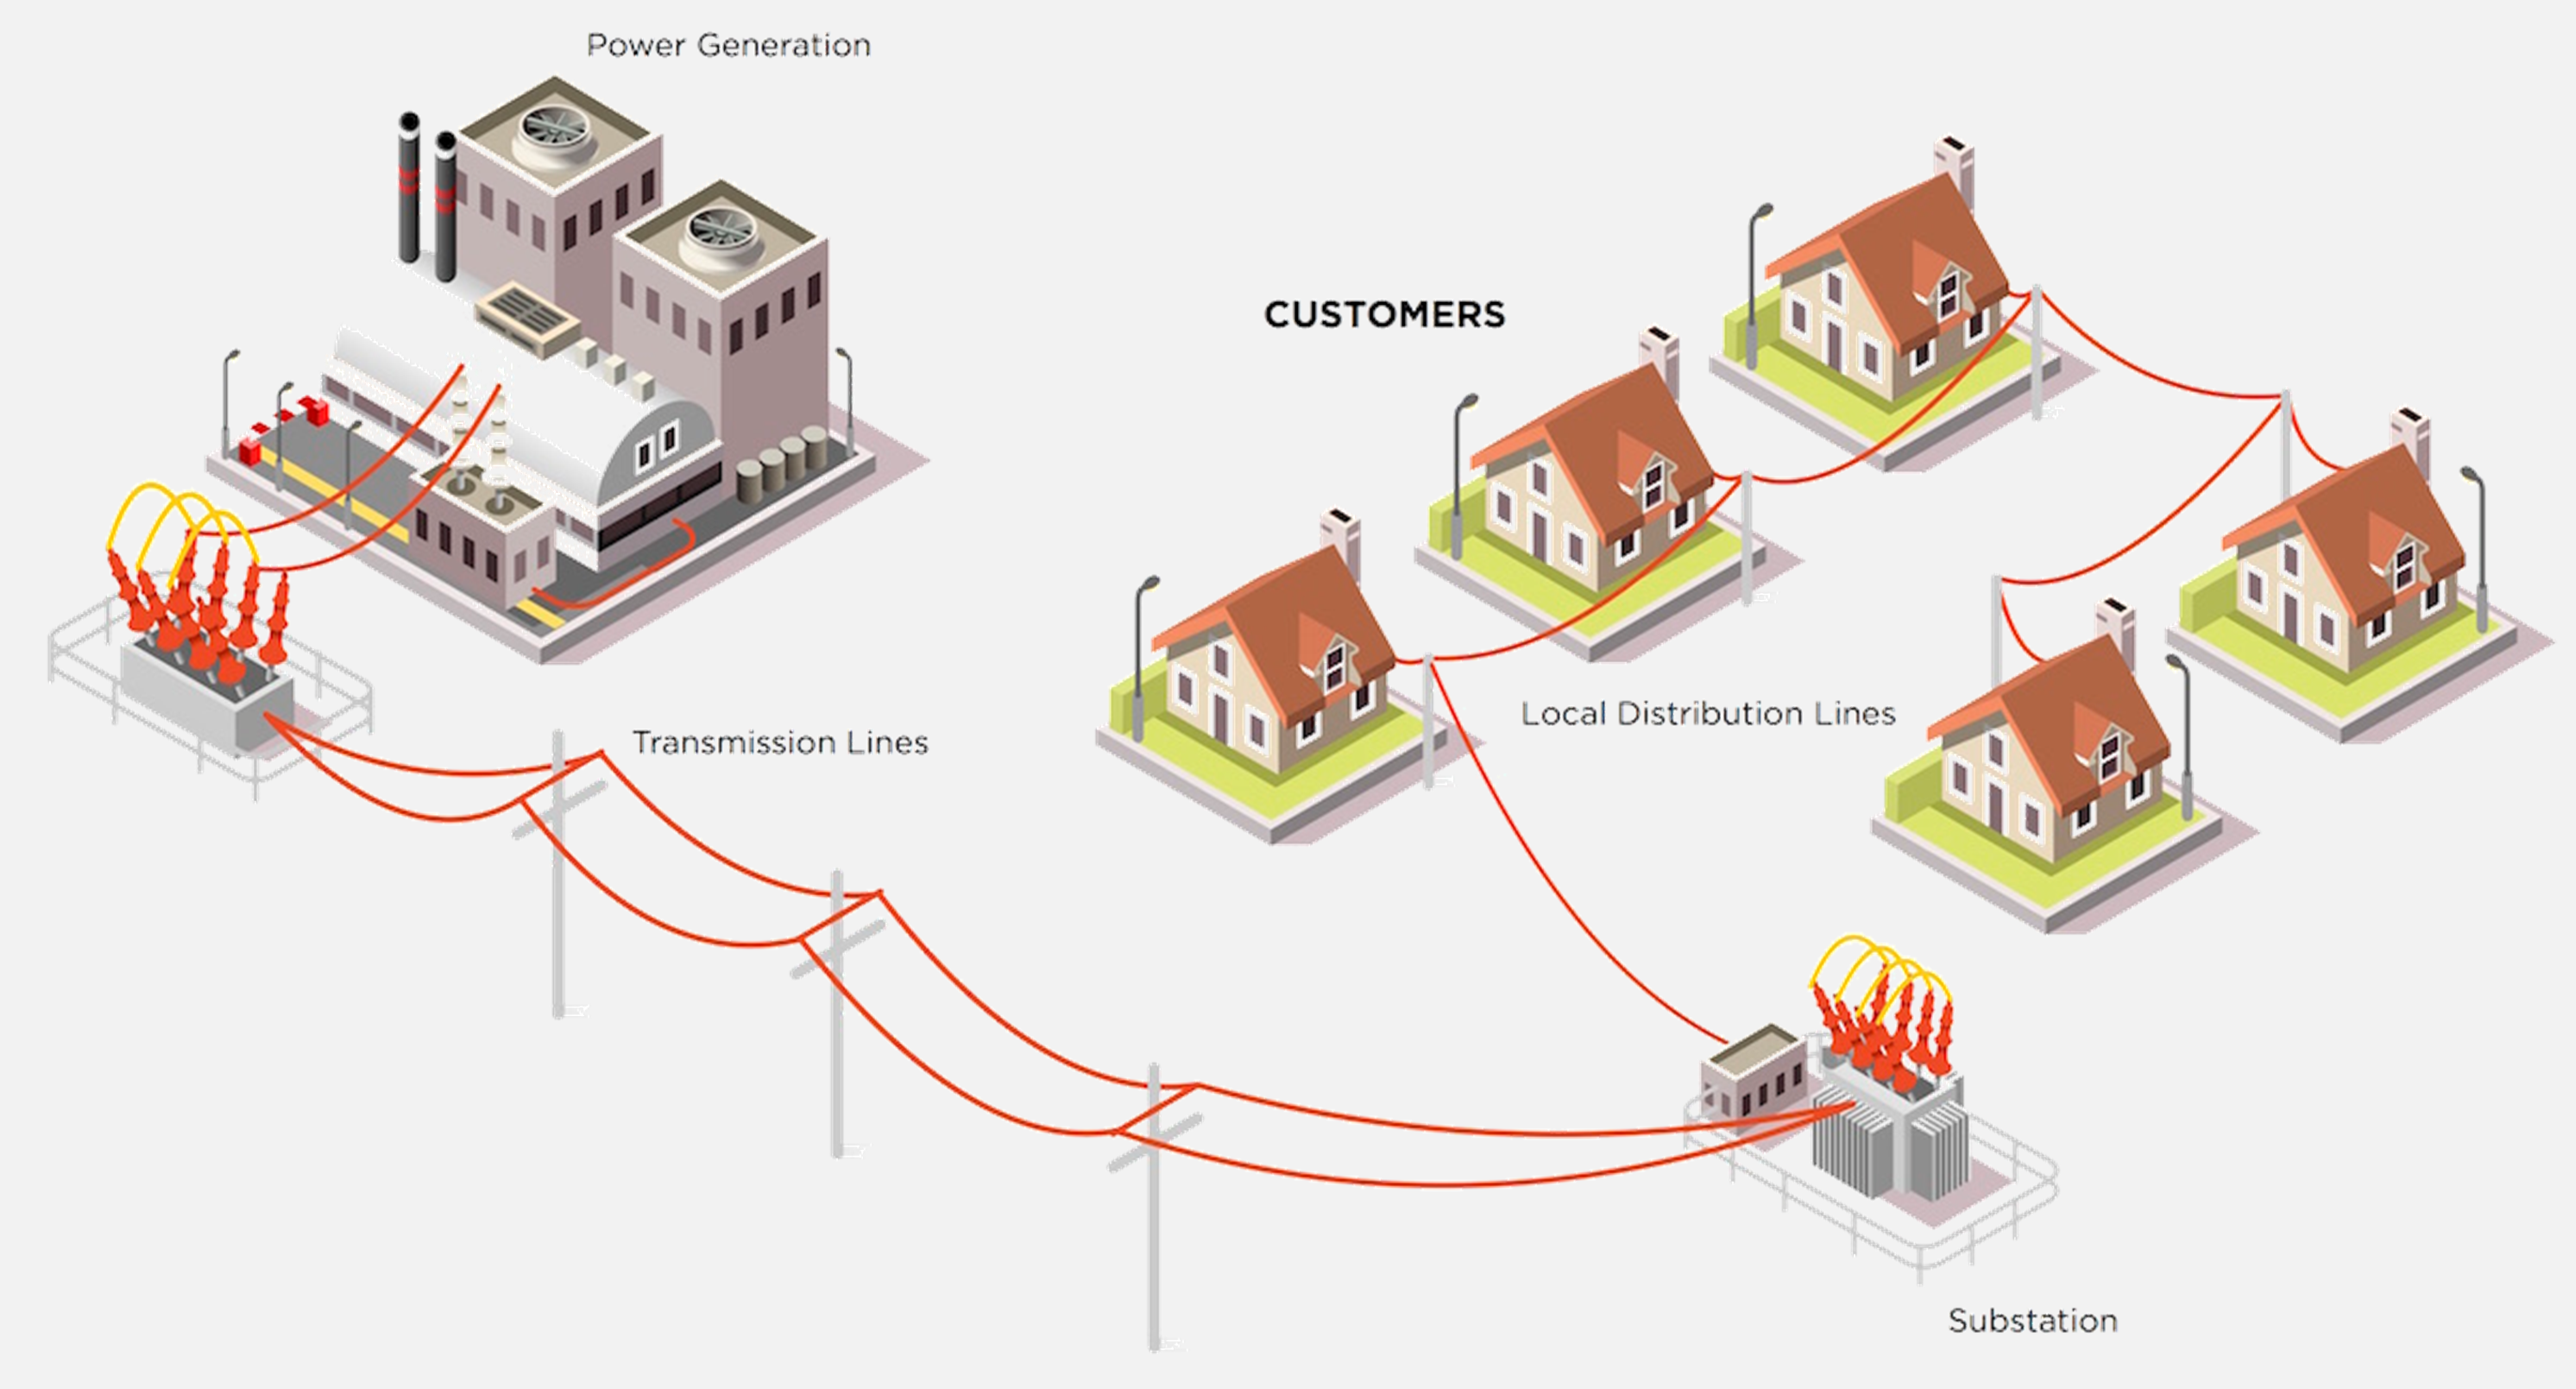
\includegraphics[width=\linewidth]{Figures/PowerSys.png}};
           \fill [draw=none, fill=white, fill opacity=0.7] (B.north west) -- (B.north east) -- (B.south east) -- (B.south west) -- (B.north west) -- cycle;
 
    \end{tikzpicture} 
    \end{backgroundblock} 

\logo{%
    
\includegraphics[width=3cm,height=3cm,keepaspectratio]{ntnulogo_eng}~%
}


\author{Salman Zaferanlouei}
\institute{NTNU{\\ \vskip 1cm} \scalebox{1.5}{\insertlogo}}
\date{\today}









\begin{document}
\begin{frame}
\titlepage
\end{frame}
%%%%%%%%%%%%%%%%%%%%%%%%%%%%%%%%%%%%%%%%%%
%%%%%%%%%%%%%%%%%%%%%%%%%%%%%%%%%%%%%%%%%%
%%%%%%%%%%%%%%%%%%%%%%%%%%%%%%%%%%%%%%%%%%
%%%%%%%%%%%%%%%%%%%%%%%%%%%%%%%%%%%%%%%%%%
\begin{frame}{Content}
\begin{itemize}
\item \textbf{Purpose:} Understanding of fast frequency reserve and current practice in Norway
\item \textbf{Time}: 45 min
\item \textbf{Target:} Public Audience
\item \textbf{How:} 
\end{itemize}
\begin{center}
\begin{tabular}{|l|} 
\hline
\rowcolor{Gray} \textbf{Inertia:} Physics of the power system \\
 \textbf{checkpoint I}\\
 \rowcolor{Gray} \textbf{TSO (Statnett):} Pilot Project 2018\\
 \textbf{checkpoint II}\\
 \rowcolor{Gray} \textbf{Concluding Remarks}\\
\hline
\end{tabular}
\end{center}



\end{frame}
%%%%%%%%%%%%%%%%%%%%%%%%%%%%%%%%%%%%%%%%%%
%%%%%%%%%%%%%%%%%%%%%%%%%%%%%%%%%%%%%%%%%%
%%%%%%%%%%%%%%%%%%%%%%%%%%%%%%%%%%%%%%%%%%
%%%%%%%%%%%%%%%%%%%%%%%%%%%%%%%%%%%%%



%%%%%%%%%%%%%%%%%%%%%%%%%%%%%%%%%%%%%%%%%%
%%%%%%%%%%%%%%%%%%%%%%%%%%%%%%%%%%%%%%%%%%
%%%%%%%%%%%%%%%%%%%%%%%%%%%%%%%%%%%%%%%%%%
%%%%%%%%%%%%%%%%%%%%%%%%%%%%%%%%%%%%%%%%%%


%%%%%%%%%%%%%%%%%%%%%%%%%%%%%%%%%%%%%%%%%%
%%%%%%%%%%%%%%%%%%%%%%%%%%%%%%%%%%%%%%%%%%
%%%%%%%%%%%%%%%%%%%%%%%%%%%%%%%%%%%%%%%%%%
%%%%%%%%%%%%%%%%%%%%%%%%%%%%%%%%%%%%%%%%%%
\section{Checkpoint II}
\begin{frame}{Checkpoint II}
\centering \begin{block}{}
\textbf{Summary:}
\end{block} 
\end{frame}

\begin{frame}{Summary}
\begin{block}{Highlights}
{\scriptsize
\begin{itemize}
\item<1-> Amount of inertia in the synchronous power system is proportional to the amount of rotating mass of synchronous generators and machines.
\item<2-> Massive integration of renewable energy generations, decommissioning of thermal and nuclear power plants (with synchronous generators), more and more dependence on HVDC import/export, all are parts of the road map toward expected near future.
\item<3-> TSO have an important role in shaping new emerging markets, by opening dialogue with market players and introduce flexibility in a socio-economical manner.
\item<4-> Pilot Project 2018:
\begin{enumerate}[I]
{\scriptsize
\item FFR is a cost efficient measure for handling of low inertia challenges.
\item Pilot project gave a profound understanding how FFR could be implemented and tested.
\item Pilot project gave an overview of how  flexibility could contribute to power system operational security. 
}



\end{enumerate}       
\end{itemize}
}
\end{block}
\end{frame}

\begin{frame}
\centering
Thank you for your attention!\\
		\vskip 0.8cm

\centering

\includegraphics[scale=0.2]{ntnulogo_eng.png}
\end{frame} 

\end{document}


